%!TEX root =../Metcalfe+Boggs.tex

%[[Graph from Above Table  -- THIS IS NOT IN ORIGINAL PAPER]]

\begin{figure}[ht]
    \centering \small 
       \caption*{\small Graph of Ethernet Efficiency [Not in Original Paper]}
    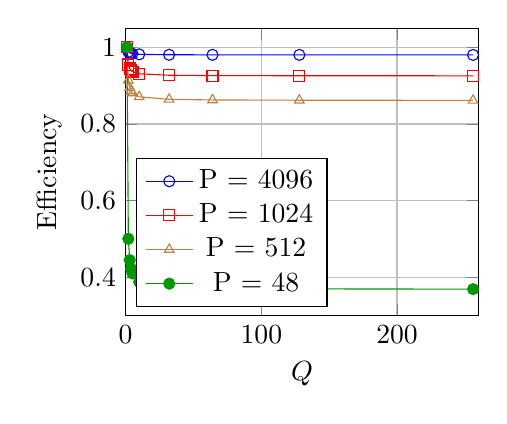
\begin{tikzpicture}
    \begin{axis}[
        width=0.5\textwidth,
        xlabel={\(\displaystyle Q\)},
        ylabel={Efficiency},
        xmin=0, xmax=260,
        ymin=0.3, ymax=1.05,
        legend pos=south west,
        grid=both
    ]
    
    %-- P = 4096
    \addplot[
        mark=o,
        blue
    ]
    coordinates {
        (1,1.0000)
        (2,0.9884)
        (3,0.9857)
        (4,0.9842)
        (5,0.9834)
        (10,0.9818)
        (32,0.9807)
        (64,0.9805)
        (128,0.9804)
        (256,0.9803)
    };
    \addlegendentry{P = 4096}
    
    %-- P = 1024
    \addplot[
        mark=square,
        red
    ]
    coordinates {
        (1,1.0000)
        (2,0.9552)
        (3,0.9447)
        (4,0.9396)
        (5,0.9367)
        (10,0.9310)
        (32,0.9272)
        (64,0.9263)
        (128,0.9259)
        (256,0.9257)
    };
    \addlegendentry{P = 1024}
    
    %-- P = 512
    \addplot[
        mark=triangle,
        brown
    ]
    coordinates {
        (1,1.0000)
        (2,0.9143)
        (3,0.8951)
        (4,0.8862)
        (5,0.8810)
        (10,0.8709)
        (32,0.8642)
        (64,0.8627)
        (128,0.8620)
        (256,0.8616)
    };
    \addlegendentry{P = 512}
    
    %-- P = 48
    \addplot[
        mark=*,
        green!60!black
    ]
    coordinates {
        (1,1.0000)
        (2,0.5000)
        (3,0.4444)
        (4,0.4219)
        (5,0.4096)
        (10,0.3874)
        (32,0.3737)
        (64,0.3708)
        (128,0.3693)
        (256,0.3686)
    };
    \addlegendentry{P = 48}
    
    \end{axis}
    \end{tikzpicture}
%    \caption*{\small Ethernet Efficiency vs.$Q$ for Different Packet Sizes $P$}
    \label{fig:ethernet-efficiency-plot}
\end{figure}
